\documentclass[12pt]{article}
\usepackage[utf8]{inputenc}
\usepackage[T1]{fontenc}
\usepackage{amsmath,amsfonts,amssymb}
\usepackage{graphicx}
\usepackage{a4wide}
\usepackage{hyperref}
%\usepackage[style=numeric-comp]{biblatex}
\usepackage{enumerate}

\newcommand{\D}{{2^Q}}
\newcommand{\bw}{\mathbf{w}}
\newcommand{\bwT}{\mathbf{w}^\mathsf{T}}
\newcommand{\T}{^\mathsf{T}}
\newcommand{\bphi}{\boldsymbol{\varphi}}
\newcommand{\bx}{\mathbf{x}}
\newcommand{\bc}{\mathbf{c}}
\newcommand{\bd}{\mathbf{d}}
\usepackage{graphicx}
\usepackage{wrapfig}
\usepackage{subcaption}
%\usepackage{latexsym}

%\newcommand{\bX}{\mathbf{X}}
%\newcommand{\bv}{\mathbf{v}
%\newcommand{\bp}{\mathbf{p}}
%\newcommand{\by}{\mathbf{y}}
%\newcommand{\beps}{\boldsymbol{\epsilon}}

\begin{document}
\begin{center}
{\Huge\bf Collision-free RFID stock inventory}% Collided birthdays are welcome!} % Signal separation
\end{center}
%\author{Vadim Strizhov}%\footnote{E-mail: vadim.vct@gmail.com}}

\begin{quote}
During inventory in a densely packed stock, multiple radio-frequency data transmitters often interfere with each other, leading to signal collisions. This reduces the efficiency of inventory. We present a method to resolve these collisions. The good news: despite these collisions, the items can still be identified, and their signals can be reconstructed. This advancement greatly enhances the performance of radio-frequency identification (RFID) systems.
%During the inventory of a crowded stock, multiple radio-frequency data transmitters often collide. It reduced number of goods in the stock to make fast inventory. We describe ways to resolve these collisions. The good news: no matter the collision, the goods could be identified. The signals could be reconstructed. It significantly ameliorates the radio-frequency identification systems.
\footnote{Vadim Strizhov, \href{mailto:vadim.vct@gmail.com}{\texttt{vadim.vct@gmail.com}}, 18/03/2025}

\bigskip
\noindent \textbf{Keywords:} RFID; I/Q data;  aloha collision; signal separation; self-modeling regression
\bigskip
\end{quote}

\section{The probability of collision-free inventory}

The Aloha protocol addresses the issue of overlapping replies by dividing the inventory time segment into discrete time slots. When prompted, each tag waits for a random number of time slots before responding. Due to this randomness, some time slots remain unoccupied, some contain only a single tag ID, while others may still be occupied by multiple tags.
\begin{wrapfigure}{r}{0.3\textwidth}  %
%\begin{figure}[!tb]
\centering
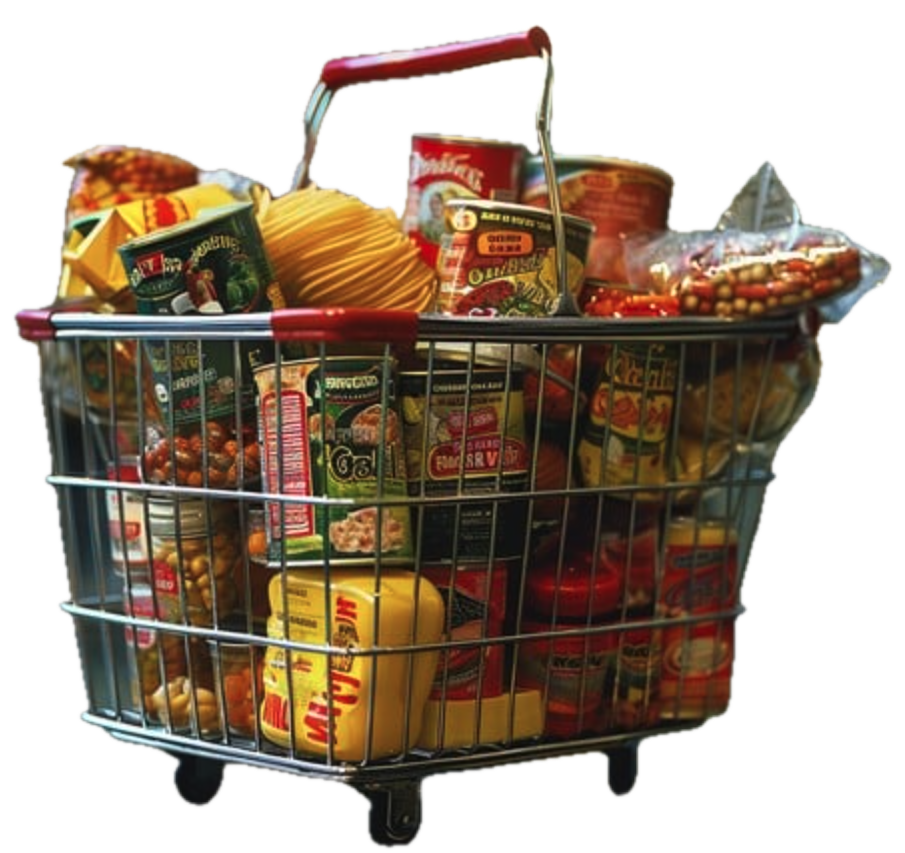
\includegraphics[width=\linewidth]{fig_shopping-cart}
\caption{The goal is to inventory over 1,000 tags at once.}
\label{fig:pr_p0}
%\end{figure}
\end{wrapfigure}
The Aloha protocol resolves a mixture of replies: the inventory time-segment splits into time-slots.  At request, each tag waits a random number of time slots and replies. 
Due to this randomness, some  time slots are left  unoccupied, some time slots keep a single tag ID, but some are still occupied by several tags.  Can we avoid collisions in one inventory cycle? The problem of estimation of probability that two tags hit one slot is called \emph{the birthday paradox}~\cite{Santos2015,Mosteller1962}. What is probability of a two people have their birthdays in the same day? One tag hits any of~$D$ slots with the probability of~$\frac{1}{D}$. Two tags do not hit the same slot with the probability~$1-\frac{1}{D}$. The third tag cannot hit both occupied slots, so the probability is
\[
\frac{D-1}{D} \frac{D-2}{D} = \left(1-\frac{1}{D}\right) \left(1- \frac{2}{D}\right).
\] 
So for given~$D$ slots,  the probability that none of~$N$ tags do not collide is
\[
\frac{D!}{D^N(D-N)!}.
\] 
Figure~\ref{fig:pr_collision-free} shows that the probability of successful inventory is small for any reasonable number of tags. So if the shopping cart has over 100 items with tags, most likely there is collision even for a long inventory cycle. See the green and red lines. 
\begin{figure}[!tb]
\centering
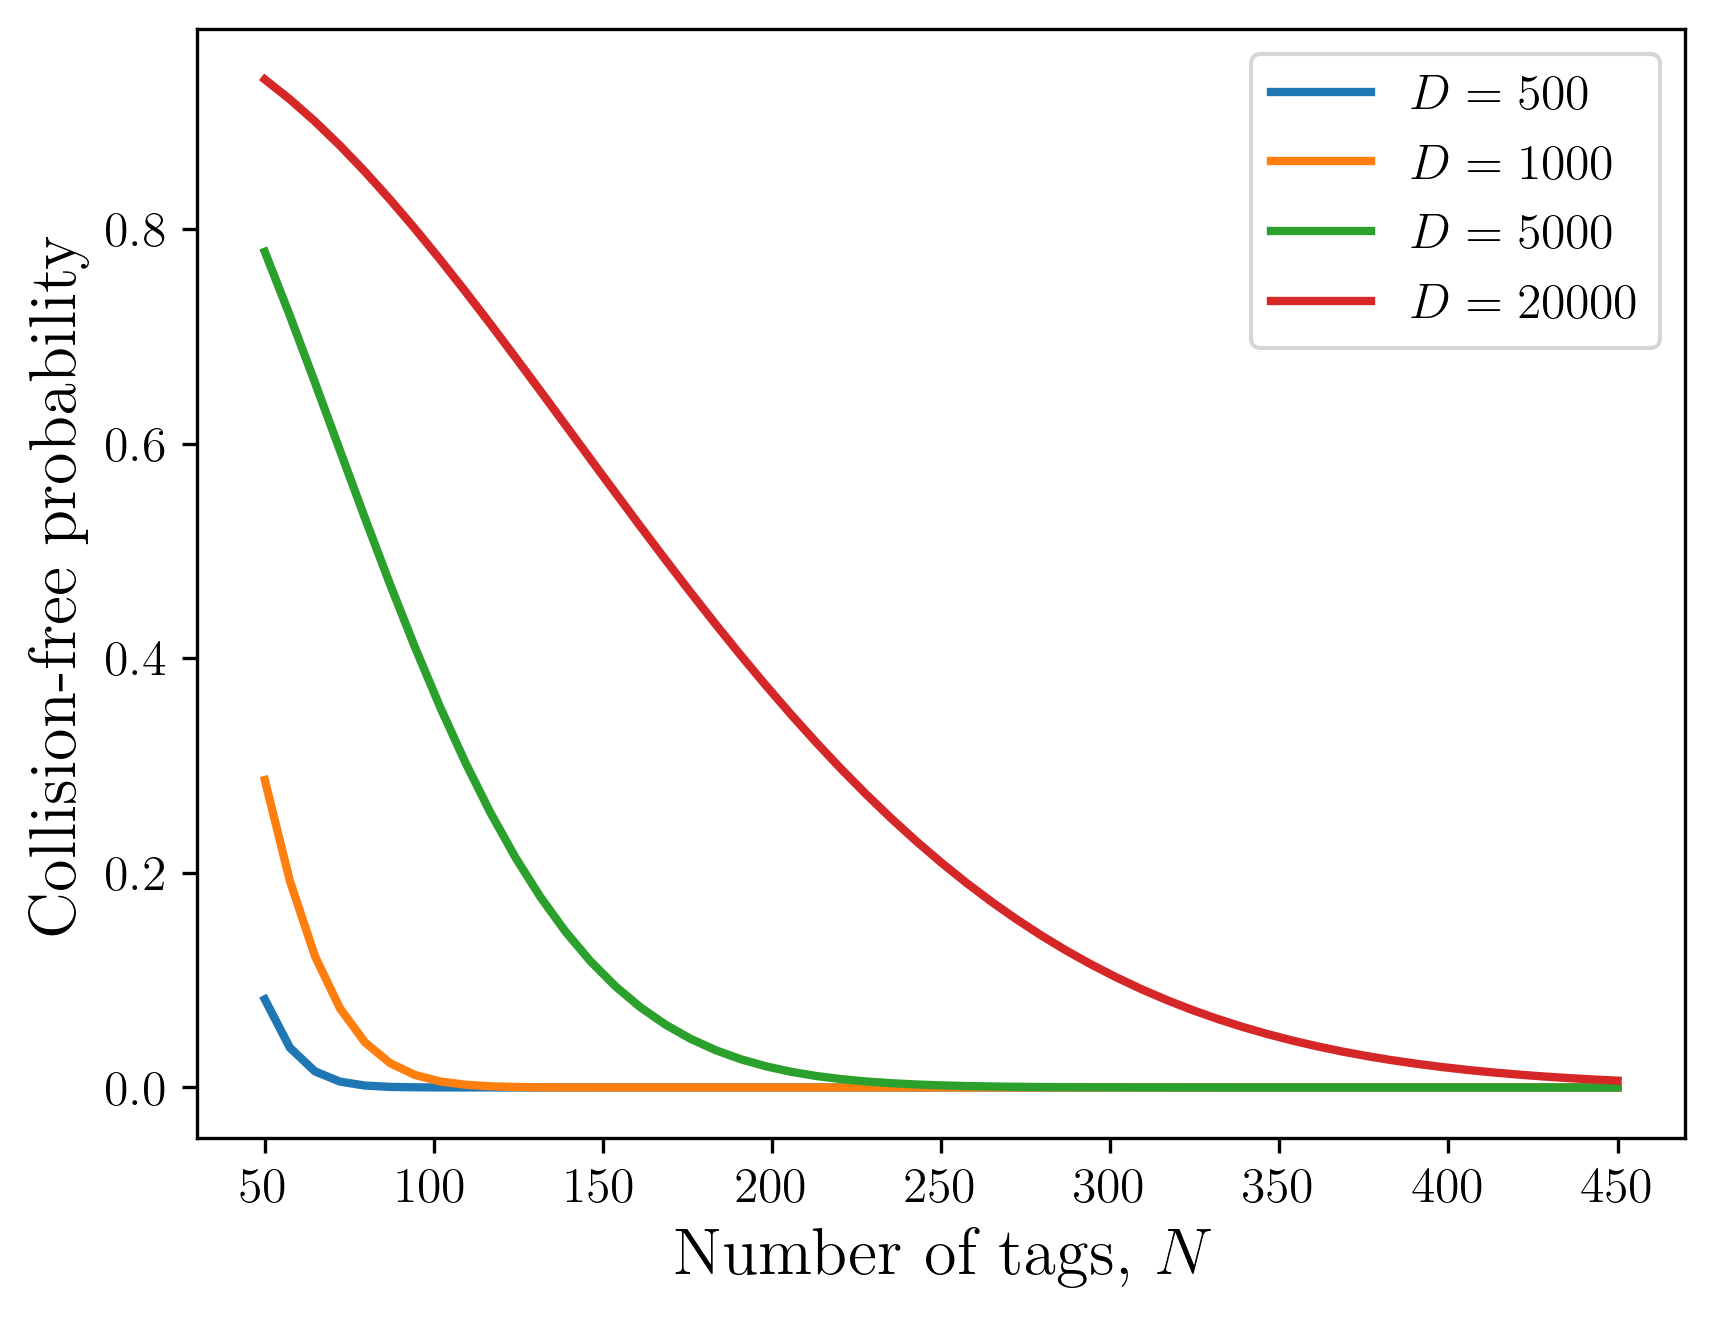
\includegraphics[width=0.5\textwidth]{fig_collision_free}
\caption{The probability of collision-free inventory of any of $N$ given $D$ time-slots.}
\label{fig:pr_collision-free}
\end{figure}

If, with an insufficiently small number of slots, there is no initial period where the probability of getting two transmitters in one slot increases. That is, if there are enough transmitters to overlap at all, they will \emph{immediately start crowding} into multiple transmissions per slot.

Briefly, \emph{the collision is inaviodable in one inventory cycle.}
%Though the probability of collision of many tags is relatively insignificant, the probability of experience a collision during a single inventory cycle is real thing and it makes our main question important. 

\section{Inphase-Quadrature Data signal self-modeling}
\begin{wrapfigure}{r}{0.2\textwidth}  %\begin{figure}[!tb]
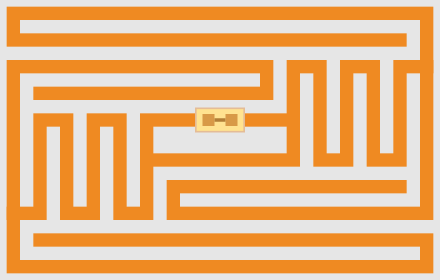
\includegraphics[width=\linewidth]{EPC-RFID-TAG.svg.png}
\caption{A tag emits a UHF signal through its antenna.}
\label{fig:antenna}%\end{figure}
\end{wrapfigure} 
The collision should be detected to avoid inventory errors. But there is no error in the signals, reconstructed after the collision. So we suppose two or more tags transmit at the same time. The inventory reader decodes the high-frequency signal into the I/Q data signal (In-phase/Quadrature). This signal carries two time series, real and imaginary. Denote these time series by~$\mathbf{x}$, a vector in the complex space. 

Since the tags are located in the different parts of shopping cart its signal is varied by phase and amplitude. Figure~\ref{fig:projected_shift} shows the same signal with the phase and amplitude modifications. The self-regression model approximates these signals with only two parameters: scale and shift.

\begin{figure}[!tp]
\centering
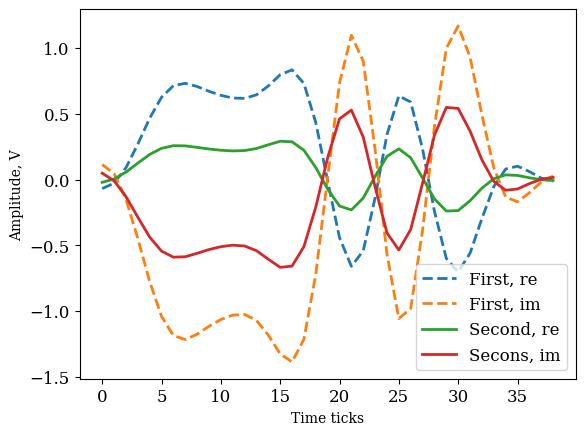
\includegraphics[width=0.45\textwidth]{fig_amplitude_scaled_distance}
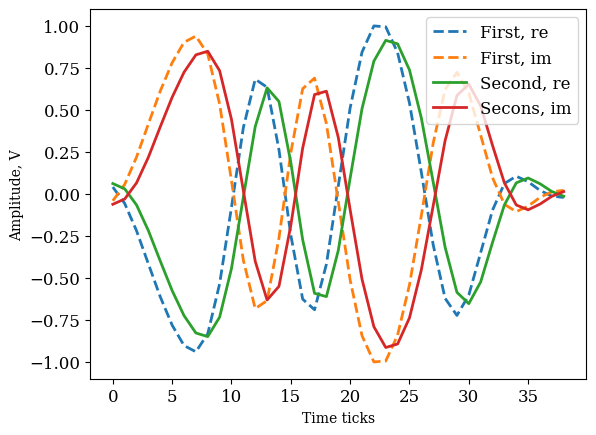
\includegraphics[width=0.45\textwidth]{fig_centroid_still_in_cluster}
\caption{The self-modeling regression regresses the first signal to the second (left), while shifting the phase of the whole I/Q data signal to find the best fit (right). The legend shows the real and imaginary parts of the complex signal.}
\label{fig:projected_shift}
\end{figure}

The self-modeling regression approximates the signal~$\bx$ with the standard signal~$\bc$ (call it the centroid) as
\[
\hat{\mathbf{c}} = \text{scale} \cdot \bigl( \text{shift}(\mathbf{x})\bigr),
\]  
%\hat{\bc} = v_1 \bigl( \text{shift}(\bx, v_2)\bigr),
with two scalar parameters: scale and shift. The first parameter is calculated as the dot product ratio of the projection 
\[
\text{scale}\cdot \mathbf{x} = \frac{\mathbf{c}^\mathsf{T}\mathbf{x}}{\|\mathbf{c}\|^2}\mathbf{c}.
\]
%Note that this ratio could be negative, which is an admissible operation for the I/Q data signal. 
The second parameter calculated as an argument of minimum distance
\[
\text{shift} =\mathop{\min}\|\hat{\mathbf{c}}-\mathbf{c}\|^2.
\]
%For the simplicity of the computations and signal processing procedures, most part of the model acts in the complex space. The variables $\bx, \bd, \bc \in \mathbb{C}^T$, where~$T$ is the length of the transmitted I/Q data signal,  $\bphi, \bw \in \mathbb{R}^K$, where~$K$ is the number of centroids, and the class~$y\in\{0,1\}.$ The in-phase part of the complex vector~$\bx$ is real, while the quadrature part is imaginary.

%Figure~\ref{fig:projected_shift} illustrates the self-modeling regression. The first, dashed, signal is the centroid, scaled to 1\,V, and the second, solid, signal is modified to approximate the centroid.

The result of self-modeling is shown in Figure~\ref{fig:cluster}
\begin{figure}[!tp]
\centering
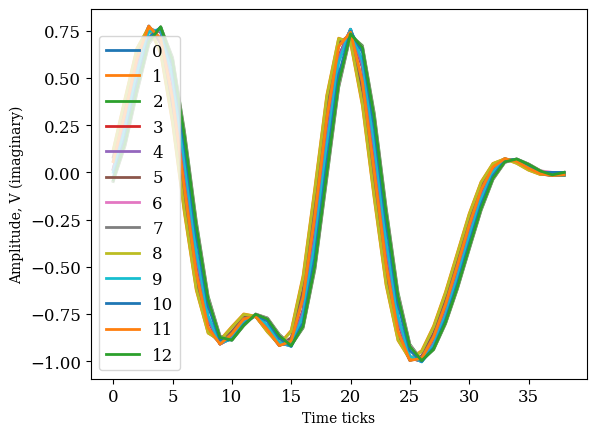
\includegraphics[width=0.45\textwidth]{fig_cluster}
\caption{After the self-modeling regression, twelve different transmissions became similar (imaginary part is shown). The figure shows the cluster of transmitted signals with the same message without noise. They scaled to the same shift phase and amplitude. }
\label{fig:cluster}
\end{figure}

Briefly, \emph{self-modeling unifies the signal shape} of  I/Q data, and it makes it a tool to analyze the signal mixtures. 
 
\begin{figure}[!t]
\centering
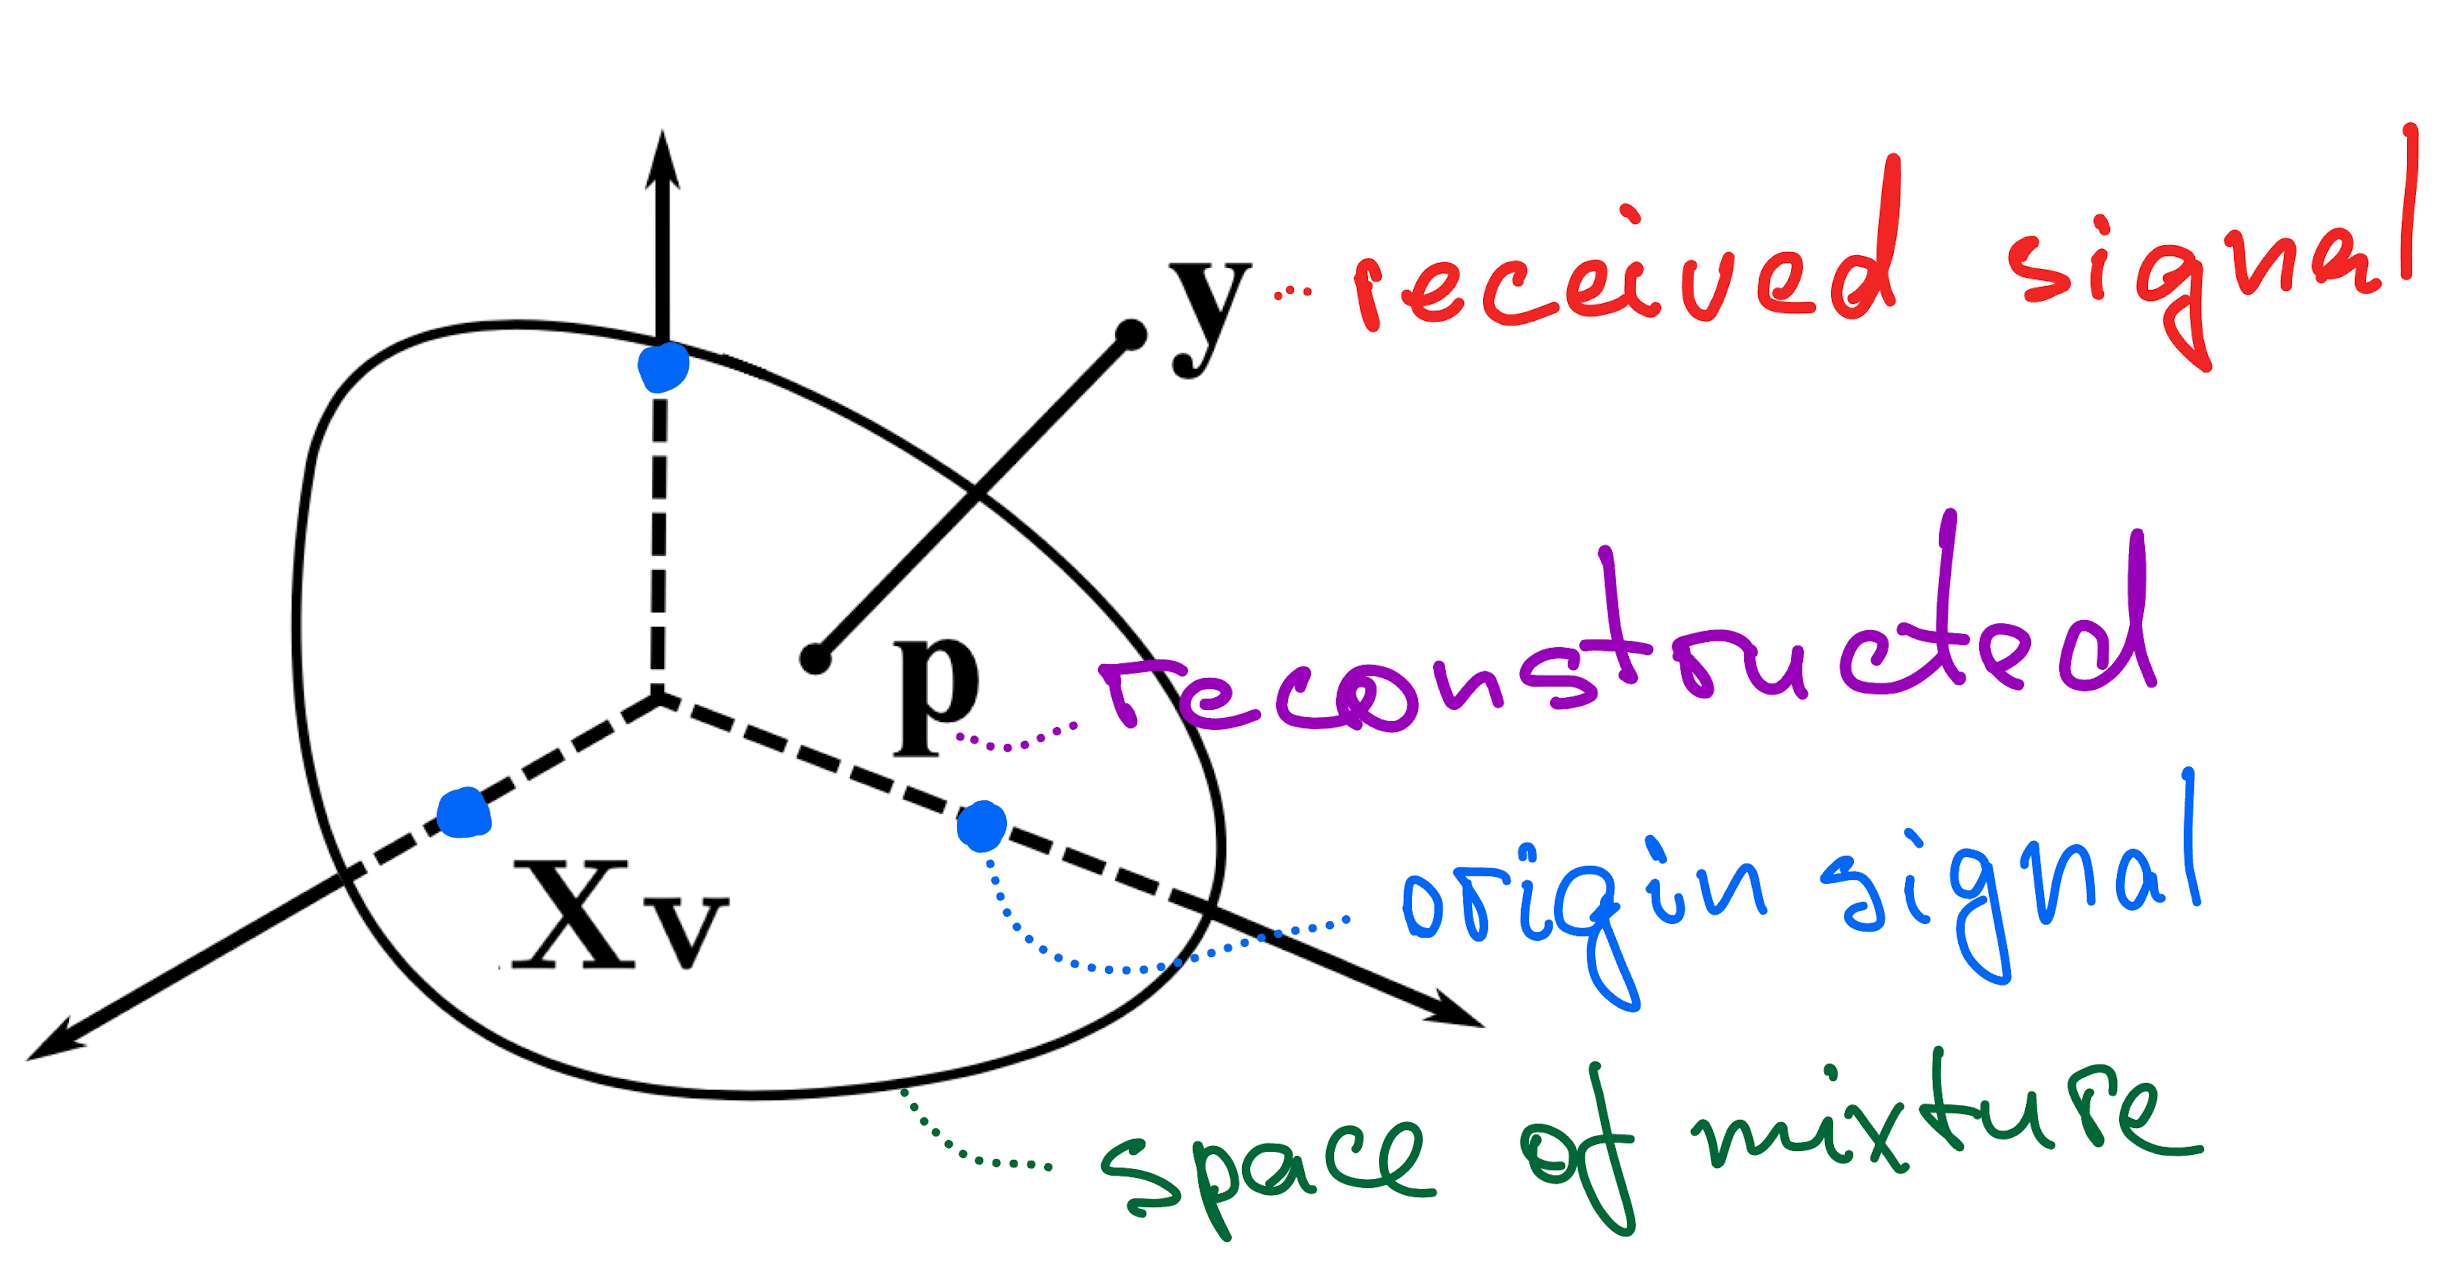
\includegraphics[width=0.5\textwidth]{fig_LSProj_hand}
\caption{Two or more signals mix proportionally to their attenuation. It defines the vector span in the space of I/Q data signals. The vector~$\mathbf{v}$ is the weights of the linear combinations of the signals. The vector~$\mathbf{p}$ is the orthogonal projection to the span~$\mathbf{X}\mathbf{v}$. The vector~$\mathbf{y}$ is the mixture of signals and the added noise to be reconstructed. The basis of~$P$ is independent (the transmitters can not send the same data) I/Q data 
signals~$\mathbf{x}_1,\ldots,\mathbf{x}_P$ form the matrix~$\mathbf{X}=[\mathbf{x}_1,\ldots,\mathbf{x}_P]$ as its columns.}
\label{fig:lsq}
\end{figure}

\section{Collision does not matter for the separated signals}
When two or more tags hit the same time slot, their signals mix. Due to the various antenna orientations, they mix with different coefficients.  For~$n$ tags denote the coefficients~$[v_1, \dots, v_n]$. The received noisy mixture~$\mathbf{y}$ approximated the weighted I/Q data signals in the best way:
\[
\mathbf{y} \approx \mathbf{p} = v_1 \bx_1 + \dots + v_n \bx_n = \mathbf{X}\mathbf{v}
\] 
%\[ \by \leadsto \mathbf{p} = v_1 \bx_1 + \dots + v_n \bx_n = \bX\bv \] 
The columns of the matrix~$\mathbf{X}$ are the stacked I/Q data signals. 
The coefficients~$\mathbf{v}$ and their number~$n$ are unknown. But for any mixture coefficients, the signals of collided tags are in the subspace of the space of the matrix~$\mathbf{X}$. Using the self-regression model, find the source signals as the nearest linear combination to the received mixture, see Figure~\ref{fig:lsq}.

\begin{figure}[!htp]
\centering
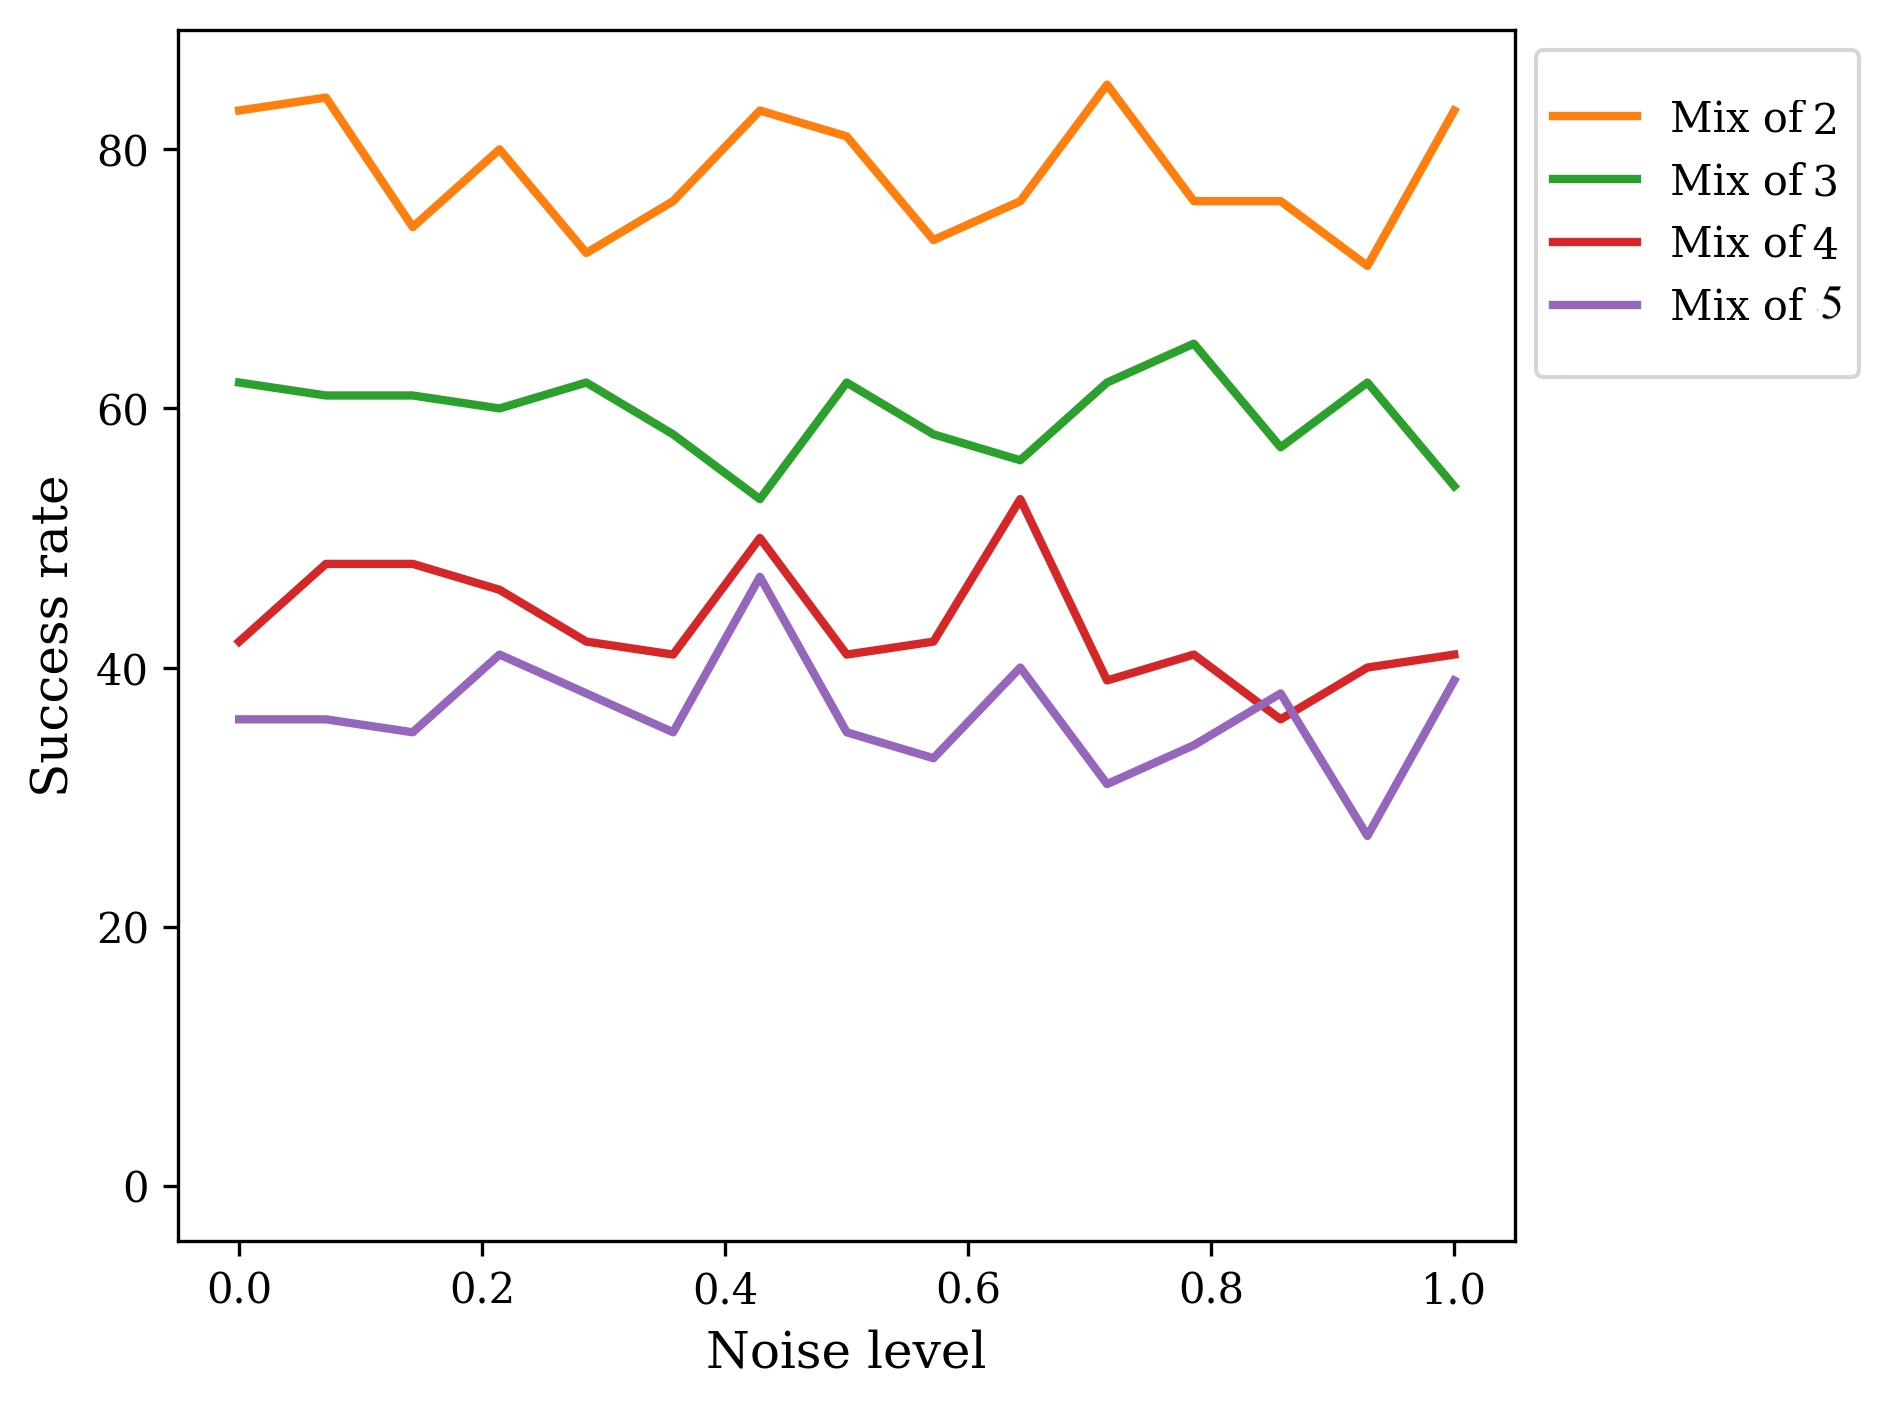
\includegraphics[width=0.6\textwidth]{fig_mix_one.png}
\caption{Each line is the number of successfully recognized IDs of the tags after the signal reconstruction. The x-axis shows level of noise from the expected standard deviation to zero. The y-axis shows the proportion of separated signals.}
\label{fig:separation}
\end{figure}
There is no need to use methods like blind signal separation. The self-modeling regression works even for a single-antenna reader. 

Figure~\ref{fig:separation} shows that the most expected types of collision: from two to five three tags hit the same slot. It delivers great I/Q data identity reconstruction.

%Briefly, \emph{collision does not matter for the separated signals}. 

\section{Development of the I/Q data separation model}
\begin{enumerate}
\item Run the code and \href{https://github.com/vadim-vic/Signal-separation}{report on the collision reconstruction} at \href{https://github.com/vadim-vic/Signal-separation}{github.com/vadim-vic/Signal-separation}. 
\item Read \href{https://github.com/vadim-vic/Signal-separation/blob/main/latex/CollisionDetector.pdf}{the report on the collision detection}.
\end{enumerate}

Though the developed model is portable to an RFID reader, there are ways to improve the signal separation. The methods are published in our papers~\cite{Katrutsa2017,Katrutsa2015}:
\begin{enumerate}
\item \href{https://doi.org/10.1016/j.eswa.2017.01.048}{Comprehensive study of feature selection methods to solve multicollinearity problem} // Expert Systems with Application, 2017
\item \href{https://doi.org/10.1016/j.chemolab.2015.01.018}{Stress test procedure for feature selection algorithms} // Chemometrics and Intelligent Laboratory Systems, 2015
\end{enumerate}

The further models include analysis of mixture in the high-frequency domain under signal interference conditions.

\bibliographystyle{unsrt}
\bibliography{CollisionDetector}
\end{document}





